\chapter{Límite Continuo}\label{cap.continuo}

En esta sección se va a estudiar la {\it función-$\zeta $} en el limite $L \rightarrow \infty$, donde $\zeta  (s)$ va a quedar definida por
\begin{equation}
	\zeta (s) = \int _{0} ^{\infty} \rho (x) \ \left( \frac{x}{\mu } 			\right) ^{-2 s} dx
\, ,	
\label{eq.zeta.continuo}
\end{equation}
donde $\rho(x) $ representa la densidad de autovalores. Para llegar a esta representación se va a utilizar la representación integral (\ref{asd}) tal como se utilizó en los capítulos \ref{seq.2.com} y  \ref{sec.finita.compleja}
\begin{equation}
\zeta (s) = 
\frac{1}{2 \pi i} 
\int _{\mathcal{C}}
\frac{M ' ( z ) }{ M ( z ) } z ^{-2s} d z = 
\frac{1}{2 \pi i} 
\int _{\mathcal{C}}
\partial _z \ \log 	M(z)  z ^{-2s} \ dz
	\, ,
	\tag{\ref{asd}}
\end{equation}
pero a diferencia de estos capítulos, el camino a utilizar es el que está representado en la imagen \ref{fig.izquierda_2} cuyos segmentos pueden parametrizarse de la forma
\begin{equation}
z(x) =  
	  \begin{cases} 
      x + i \epsilon  &  x \in [x _0, \infty] \\
      x - i \epsilon  &  x \in  [ x_0, \infty) \\
      x _0 + i x	  &  x \in [-\epsilon,\epsilon]
   \end{cases}
\label{eq.para.con}
\end{equation}
De (\ref{larga}) se puede ver que $S _1,S _2 \rightarrow 1$ cuando $L \rightarrow \infty$, por lo tanto se utilizará la función $M (z)$ definida en (\ref{eq.completa}).


Al igual que en los capítulos \ref{seq.2.com} y  \ref{sec.finita.compleja} se va a generar un termino exponencialmente decreciente, el cual en este caso va a tender a cero en el límite $L \rightarrow \infty$. Las tres integrales provenientes de la parametrización (\ref{eq.para.con}) quedan determinadas por 
\begin{align}
\zeta (s) =& \\
& +
\nonumber
	\frac{ 1 }{2 \pi i}  
	\int _{\infty} ^{x _0} 
	\left( \frac{x}{\mu} \right) ^{-2s} \times
\\
&
\nonumber
	\times
	\left( +
	\frac{i \alpha}{2 x^2} - 
	\frac{i \alpha }{2 \lambda ^2} \log ( 2 \lambda L ) +
	\frac{i \alpha}{2 x ^2 } \psi \left( 1 + \frac{i \alpha}{2 x} \right) +
	\epsilon _L
	\right)
	d x
\label{int1}	
\\
\nonumber
& +
	\frac{ 1 }{2 \pi i}  
	\int _{x _0} ^{\infty} 
	\left( \frac{x}{\mu} \right) ^{-2s}
	\times
\\
&
	\times	
	\left( -
	\frac{i \alpha}{2 x^2} + 
	\frac{i \alpha }{2 \lambda ^2} \log ( 2 \lambda L ) -
	\frac{i \alpha}{2 x ^2 } \psi \left( 1 + \frac{i \alpha}{2 x} \right) +
	\epsilon _L
	\right)
	d x
\nonumber
\\
& +
\nonumber
	\frac{ 1 }{2 \pi i}	
	\int _{- \epsilon} ^{\epsilon}
	O (\epsilon) \, dx
\, .	
\end{align}
donde $\lim \limits _{L \rightarrow \infty} \epsilon _L = 0$, por lo tanto la última integral no se tendrá en cuenta. Obteniendo para $\zeta(s) $
\begin{align}
&
	\zeta (s)=
	\frac{L }{\pi}
	\int _ {x_0} ^{\infty} \left( \frac{x}{\mu} \right) ^{-2s} dx
\\	 
& 
\nonumber
	+
	\frac{\alpha }{2 \pi } \int _{x_0} ^{\infty} 
	\left( \frac{x}{\mu} \right) ^{-2s}
	\left(-
	\frac{1}{ x ^2} +
	\frac{\log \left( 2 x L \right) }{x ^2}  -
	\frac{1}{ 2 x ^2 } 
	\left(
	\psi \left( 1 + \frac{i \alpha}{2  x} \right) + \psi \left( 1 - \frac{i \alpha}{2 x} \right) 
	\right)
	\right)
	d x
	\, .
\end{align}
Realizando las integrales término a término se obtiene:
\begin{align}
	\zeta (s)=
&
\nonumber
	\frac{L  \mu ^{2s} x _0 ^{1-2s} }{2 \pi \left( s- \frac{1}{2} \right)}  + 
	\frac{\alpha \mu ^{2s} x _{0} ^{-2s-1} }{2 \pi} 
	\left( 
	\frac{1}{4 \left(s+ \frac{1}{2} \right) ^2} +
	\frac{\log(2 x _0 L) -1 }{2 \left(s+\frac{1}{2} \right)} 
	\right) 
\\
-
&	
	\frac{\alpha \mu ^{2s} }{4 \pi}
	\int _{x_0} ^{\infty} 
	x ^{-2s-2}
	\left(
	\psi \left( 1 - \frac{i \alpha}{2 x} \right) +
	\psi \left( 1 + \frac{i \alpha}{2 x} \right)
	\right)
	dx
\, .
\end{align}
Para calcular el último término hay distintos desarrollos en serie de la función poligamma $\psi $ que se pueden utilizar, se va a usar el desarrollo dado en \cite{Abramowitz:1974:HMF:1098650}.
\begin{equation}
\begin{array}{cc}
\psi (1+ z ) = - \gamma + \sum \limits_{n=2}^{\infty} (-1) ^n \zeta _R (n) z ^{n-1},  & |z| < 1
\, ,
\end{array}
\label{repr}
\end{equation}
con lo cual el ultimo término queda expresado de la forma
\begin{equation}
- \frac{\alpha \mu ^{2s}}{4 \pi}
\int _{x_0} ^{\infty}
\left(
-2 \gamma -
2 \sum _{n=1} ^{\infty} 
(-1) ^{n}
\zeta _R (2n+1) 
\left( \frac{\alpha}{2 x} \right) ^{2n}
\right)
x ^{-2s-2} dx
\, ,
\end{equation}
pudiendose expresar para $\zeta  (s) $ en este caso como
\begin{align}
	\zeta (s)=
&
\nonumber
	\frac{L  \mu ^{2s} x _0 ^{1-2s} }{2 \pi \left( s- \frac{1}{2} \right)}  + 
	\frac{\alpha \mu ^{2s} x _{0} ^{-2s-1} }{2 \pi} 
	\left( 
	\frac{1}{4 \left(s+ \frac{1}{2} \right) ^2} +
	\frac{\log(2 x _0 L) -1 + \gamma}{2 \left(s+\frac{1}{2} \right)} 
	\right) 
\\
+
&	
	\frac{\alpha \mu ^{2s}}{4\pi} 
	\sum _{n=1} ^{\infty} (-1) ^{n} \zeta _R (2n+1) 
	\left( \frac{\alpha}{2 } \right) ^{2n} \ \frac{x _0 ^{-2s-2n-1}}{s+n+ \frac{1}{2}}
	\, ,
\end{align}
de aquí puede verse que $ \zeta (s) $ ademas de poseer los polos en $s = \pm \frac{1}{2}$, al igual que el caso finito posee polos simples en $ s = -n - \frac{1}{2}$ que están dados por
\begin{equation}
	\left( s + n + \frac{1}{2}\right)
	\zeta \left( s \rightarrow -n - \frac{1}{2}\right) =
	\frac{(-1) ^n \zeta _R (2n+1)}{4 \pi \ 2 ^{ 2n } }
	\left( \frac{\alpha}{\mu} \right) ^{2n+1}
	\, ,
\end{equation}
tambien puede verse que el polo en $s = - \frac{1}{2}$ está dado por 
\begin{align}
	\zeta \left(- \frac{1}{2} + \epsilon \right)=
&
\nonumber
	-
	\frac{L x _0 ^2}{2 \pi \mu}+ 
	\frac{\alpha}{8 \pi \mu  \epsilon  ^2} +
	\frac{\alpha \left( \log (2 L \mu ) + \gamma -1  \right)}{4 \pi \mu  \epsilon }
\\
\nonumber
&
+
	\frac{\alpha \log \left( \frac{\mu}{x _0} \right) 	
		\left( 2 (\log ( 2 L x_0) + \gamma -1 ) + \log \left( \frac{\mu}{x _0}\right)  \right) }{4 \pi \mu}
\\
&
+	
	\frac{\alpha }{4\pi} 
	\sum _{n=1} ^{\infty} \frac{(-1) ^{n} \zeta _R (2n+1) }{n}  
	\left( \frac{\alpha}{2 x _0} \right) ^{2n}
\, ,
\end{align}
una observación es que los polos en $s = -\frac{1}{2}$ coinciden con los calculados para un intervalo $L$ finito en las expresiones (\ref{eq.result.zeta.c}) y (\ref{eq.res.1}).
Para la energía de vacío se obtiene la expresión analítica
\begin{align}
\label{eq.energia.cotinua}
	E _0 ( \epsilon ) 
&	
	=
\nonumber
	\frac{\alpha}{16 \pi  \epsilon  ^2} +
	\frac{\alpha \left( \log (2 L \mu ) + \gamma -1  \right)}{8 \pi \epsilon } -
	\frac{L x _0 ^2}{4 \pi}
\\
\nonumber
&
+
	\frac{\alpha \log \left( \frac{\mu}{x _0} \right) 	
		\left( 2 (\log ( 2 L x_0) + \gamma -1 ) + \log \left( \frac{\mu}{x _0}\right)  \right) }{8 \pi}
\\
&
+	
	\frac{\alpha }{8 \pi} 
	\sum _{n=1} ^{\infty} \frac{(-1) ^{n} \zeta _R (2n+1) }{n}  
	\left( \frac{\alpha}{2 x _0} \right) ^{2n}
\, ,
\end{align}
de aquí puede verse que además de presentarse los términos dependientes de la escala $\log ( \mu )$ se presenta una dependencia con el parámetro de corte $x _0$.
En la figura \ref{fig:vacio} se encuentra graficado el último termino de la energía de vacío en función del parámetro $x = \frac{\alpha}{x_0}$ en donde puede observarse una divergencia alrededor de $x=2$ la cual se debe a la representación (\ref{repr}).

\begin{figure}
    \centering
    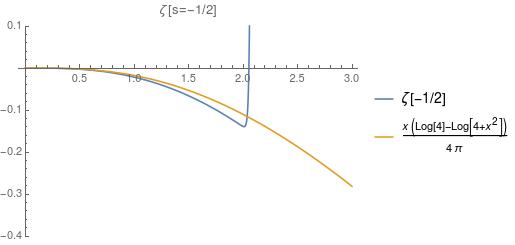
\includegraphics[scale=0.5]{Vacio.pdf}
    \caption{En esta imagen esta graficada la parte finita de la $E _0 (\epsilon) $ de la ecuación \ref{eq.energia.cotinua} en función del parámetro $x= \frac{\alpha}{x _0}$ donde se sumaron los primeros 100 términos de la serie, puede verse un claro comportamiento divergente alrededor de $x=2$}
    \label{fig:vacio}
\end{figure}



